\subsection{Spectrogram Preprocessing}\label{sec:preproc}

Before any features can be extracted, their pixel boundaries must be found.
This is a non-trivial problem due to noise and recording artefacts
that may be present in each spectrogram.
The complexity of the problem is increased by their inconsistency.

Figure~\ref{fig:sgram_noise} shows an example of a noisy spectrogram.
Notice how baseline and background noise makes it difficult to determine 
the exact boundary of some of the vocalisations.

\begin{figure}[h]
  \centering
  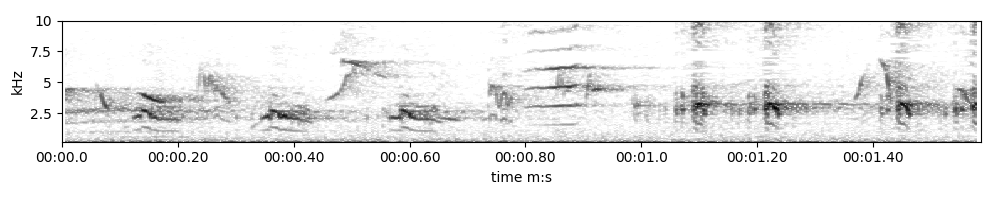
\includegraphics[width=1.0\textwidth]{noisy_sgram}
  \caption{Noisy spectrogram of a segment of a Great Reed Warbler's 
  song.}
  \label{fig:sgram_noise}
\end{figure}

Even with the metadata-based quality prefiltering done when downloading recordings from
Xeno-canto, noise levels remain at unsuitable levels for direct signal detection.

Removing noise and unwanted artefacts manually is precise, although tedious.
Because a high number of samples is required for our approach, we developed an
automatic noise reduction stage, as doing so manually would be far too
impractical at this scale.
Standard computer vision techinques for noise reduction are used, as well as
techniques for discrete object identification.

\begin{figure}[!htb]
  \centering
  \begin{subfigure}[b]{1\textwidth}
    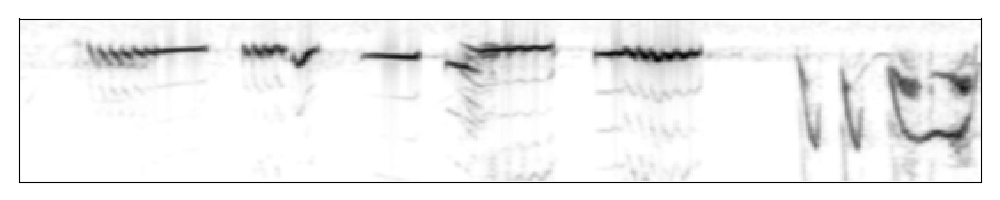
\includegraphics[width=1.0\textwidth]{pp_gauss}
    \caption{Gaussian filter, $k=5x5, \sigma=0$}
    \label{fig:preproc_vis_filter}
  \end{subfigure}
  \begin{subfigure}[b]{1\textwidth}
    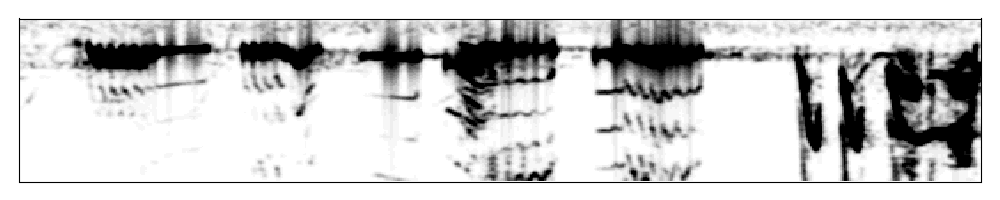
\includegraphics[width=1.0\textwidth]{pp_ttrunc}
    \caption{Otsu's threshold truncation}
    \label{fig:preproc_vis_thresh}
  \end{subfigure}
  \begin{subfigure}[b]{1\textwidth}
    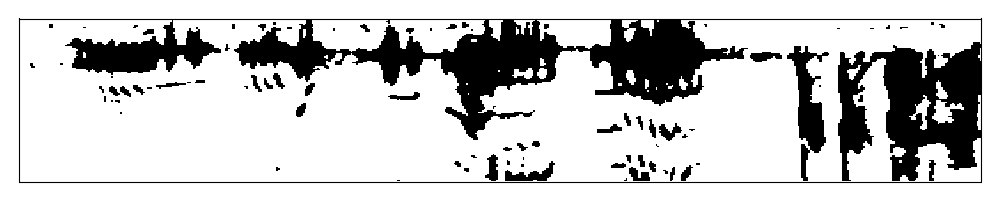
\includegraphics[width=1.0\textwidth]{pp_tbin}
    \caption{Otsu's threshold binarization}
    \label{fig:preproc_vis_thresh2}
  \end{subfigure}
  \begin{subfigure}[b]{1\textwidth}
    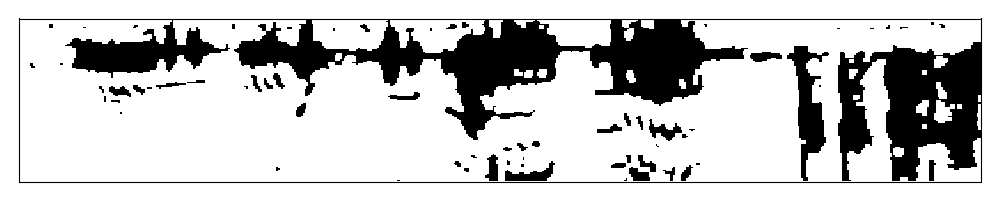
\includegraphics[width=1.0\textwidth]{pp_small}
    \caption{Dilation followed by erosion, $k=7x7$}
    \label{fig:preproc_vis_dilation1}
  \end{subfigure}
  \begin{subfigure}[b]{1\textwidth}
    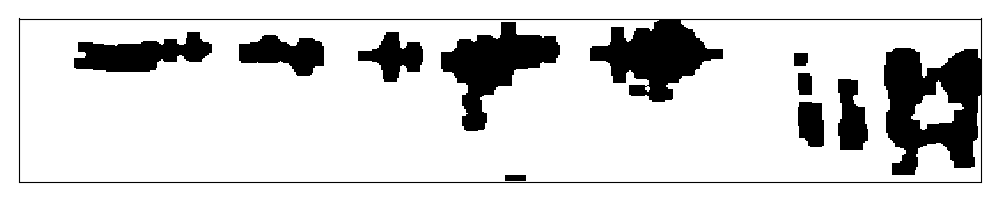
\includegraphics[width=1.0\textwidth]{pp_fill}
    \caption{Closing, 3x3 ellipse}
    \label{fig:preproc_vis_closing}
  \end{subfigure}
  \caption{Preprocessing stages in order.}
  \label{fig:preproc_vis}
\end{figure}
%taken from xc210575
\subsubsection{The mechanism}
A filter is first applied to the spectrogram, which reduces the noise in the
image by smoothing just enough until granular noise is reduced sufficiently
(Figure~\ref{fig:preproc_vis_filter}).
This is accomplished using a Gaussian filter with a 5x5 kernel and sigma of 0.
Several other filtering methods were also tested, including a median filter,
but these were not compared directly.

The image is then thresholded using a thresholding algorithm
(Figure~\ref{fig:preproc_vis_thresh}).
Otsu's binarization thresholding technique \parencite{otsu1979} was used to
select an optimal threshold value.
Because of pixel intensity inconsistencies throughout individual spectrograms,
specifically in areas where noise is prominent, an adaptive thresholding
algorithm was also tested.
This does not appear to provide generally better results.
Thresholding is performed twice, initially as a truncation method, then again
for binarization (Figure~\ref{fig:preproc_vis_thresh2}).
This appears to perform better than binarizing immediately.

Further noise reduction is then performed using dilation and erosion
(Figure~\ref{fig:preproc_vis_dilation1}),
which removes small segments and joins pixel groups which are in close proximity
to each other.
Notice that the order of operations is flipped here since we are working with
an inverted spectrogram.
A kernel size of 7x7 is used.

Most remaining holes are then filled using a closing morphology algorithm,
using an ellipse of size 3x3 (Figure~\ref{fig:preproc_vis_closing}).\\

These procedures transform the spectrogram into a binary image
consisting of discrete pixel segments.
This representation simplifies the extraction procedure as described in
Section~\ref{sec:extract}.


\subsubsection{Granularity considerations}\label{sec:granularity}
It is important to consider and evaluate the granularity to aim for when
isolating sections of song.
It is not clear if phrases perform better than syllables or elements for example.
An evaluation should therefore be performed to determine the best granularity.

Conclusive testing different granularities bears the weight of template matching
for all new templates, which is extremely time consuming.

Further, achieving consistent granularity across all spectrograms is not a trivial
task, and is certainly not possible if a single parameter set is used for
all spectrograms.

A loose aim is therefore taken to extract the smallest possible non-singular
vocalisations, as close as possible to what is defined as a syllable.
This of course does not always work, but the developed mechanism provides generally
good results.


\subsubsection{Quality and consistency}
It is difficult to arrive at a single set of optimal parameters which work
well across all spectrograms.
An adaptive method is therefore suggested (but not implemented):
Preprocessing parameters may be specified on a per-recording basis if prior
knowledge is gathered for expected vocalisation/section counts, template
dimensions, and frequency range.
Since there is no known structured source of data for this, it is necessary to
manually specify these on a per-species basis.
Alternatively a fully automatic method is conceivable by feeding back the
classification results with each granularity setting.
This however would be incredibly time consuming on standard hardware, and may
be sensitive to other factors in the classification pipeline.

Consistent quality becomes less of a concern as the number of samples used for
training increases.
It can be shown that as the sample count increases, the number of valid templates
tends to increase.
The number of noise also increases, however these do not intercorrelate as valid
templates do, and are handled well by less sensitive classifiers such as
random forests \parencite{marko2004} so long as there are not too many of them.

Quality is therefore moderated after preprocessing in the selection stage as
described in Section~\ref{sec:template_select}.

\begin{figure}[!htb]
  \centering
  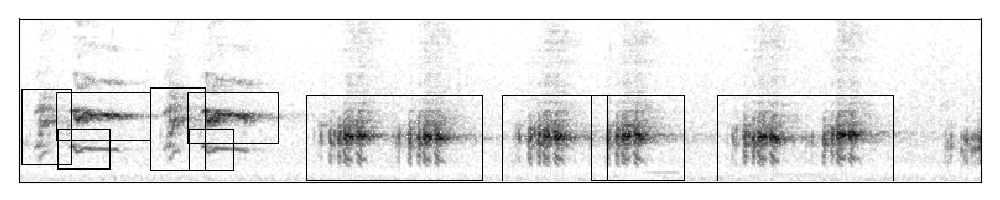
\includegraphics[width=1\textwidth]{varying_gran}
  \caption{Example of selected templates with varying granularity}
  \label{fig:varygran}
\end{figure}
